% !TEX encoding = UTF-8
% !TEX TS-program = pdflatex
% !TEX root = tesi.tex
% !TEX spellcheck = it-IT

\documentclass[10pt,                    % corpo del font principale
               a4paper,                 % carta A4
               twoside,                 % impagina per fronte-retro
               openright,               % inizio capitoli a destra
               english,                 
               italian,                 
               ]{book}    

%**************************************************************
% Importazione package
%************************************************************** 

%\usepackage{amsmath,amssymb,amsthm}    % matematica

\usepackage[T1]{fontenc}                % codifica dei font:
                                        % NOTA BENE! richiede una distribuzione *completa* di LaTeX

\usepackage[utf8]{inputenc}             % codifica di input; anche [latin1] va bene
                                        % NOTA BENE! va accordata con le preferenze dell'editor

\usepackage[english, italian]{babel}    % per scrivere in italiano e in inglese;
                                        % l'ultima lingua (l'italiano) risulta predefinita

\usepackage{bookmark}                   % segnalibri

\usepackage{caption}                    % didascalie

\usepackage{chngpage,calc}              % centra il frontespizio

\usepackage{csquotes}                   % gestisce automaticamente i caratteri (")

\usepackage{emptypage}                  % pagine vuote senza testatina e piede di pagina

\usepackage{epigraph}			% per epigrafi

\usepackage{eurosym}                    % simbolo dell'euro

%\usepackage{indentfirst}               % rientra il primo paragrafo di ogni sezione

\usepackage{graphicx}                   % immagini

\usepackage{hyperref}                   % collegamenti ipertestuali

\usepackage[binding=5mm]{layaureo}      % margini ottimizzati per l'A4; rilegatura di 5 mm

\usepackage{listings}                   % codici

\usepackage{microtype}                  % microtipografia

\usepackage{mparhack,fixltx2e,relsize}  % finezze tipografiche

\usepackage{nameref}                    % visualizza nome dei riferimenti                                      

\usepackage[font=small]{quoting}        % citazioni

\usepackage{subfig}                     % sottofigure, sottotabelle

\usepackage[italian]{varioref}          % riferimenti completi della pagina

\usepackage[dvipsnames]{xcolor}         % colori

\usepackage{booktabs}                   % tabelle                                       
\usepackage{tabularx}                   % tabelle di larghezza prefissata                                    
\usepackage{longtable}                  % tabelle su più pagine                                        
\usepackage{ltxtable}                   % tabelle su più pagine e adattabili in larghezza

\usepackage[toc, acronym]{glossaries}   % glossario
                                        % per includerlo nel documento bisogna:
                                        % 1. compilare una prima volta tesi.tex;
                                        % 2. eseguire: makeindex -s tesi.ist -t tesi.glg -o tesi.gls tesi.glo
                                        % 3. eseguire: makeindex -s tesi.ist -t tesi.alg -o tesi.acr tesi.acn
                                        % 4. compilare due volte tesi.tex.

\usepackage[backend=biber,style=verbose-ibid,hyperref,backref]{biblatex}
                                        % eccellente pacchetto per la bibliografia; 
                                        % produce uno stile di citazione autore-anno; 
                                        % lo stile "numeric-comp" produce riferimenti numerici
                                        % per includerlo nel documento bisogna:
                                        % 1. compilare una prima volta tesi.tex;
                                        % 2. eseguire: biber tesi
                                        % 3. compilare ancora tesi.tex.

\usepackage{lmodern}



%**************************************************************
% file contenente le impostazioni della tesi
%**************************************************************

%**************************************************************
% Frontespizio
%**************************************************************

% Autore
\newcommand{\myName}{Riccardo Bernucci}                                    
\newcommand{\myTitle}{Analisi, Progettazione e Implementazione di un componente Software adottando Instant Developer}

% Tipo di tesi                   
\newcommand{\myDegree}{Tesi di laurea triennale}

% Università             
\newcommand{\myUni}{Università degli Studi di Padova}

% Facoltà       
\newcommand{\myFaculty}{Corso di Laurea in Informatica}

% Dipartimento
\newcommand{\myDepartment}{Dipartimento di Matematica "Tullio Levi-Civita"}

% Titolo del relatore
\newcommand{\profTitle}{Prof.}

% Relatore
\newcommand{\myProf}{Francesco Ranzato}

% Luogo
\newcommand{\myLocation}{Padova}

% Anno accademico
\newcommand{\myAA}{2018-2019}

% Data discussione
\newcommand{\myTime}{Luglio 2019}


%**************************************************************
% Impostazioni di impaginazione
% see: http://wwwcdf.pd.infn.it/AppuntiLinux/a2547.htm
%**************************************************************

\setlength{\parindent}{14pt}   % larghezza rientro della prima riga
\setlength{\parskip}{0pt}   % distanza tra i paragrafi


%**************************************************************
% Impostazioni di biblatex
%**************************************************************
%\bibliography{bibliografia} % database di biblatex 

%\defbibheading{bibliography} {
%    \cleardoublepage
%    \phantomsection 
%    \addcontentsline{toc}{chapter}{\bibname}
%    \chapter*{\bibname\markboth{\bibname}{\bibname}}
%}

%\setlength\bibitemsep{1.5\itemsep} % spazio tra entry

%\DeclareBibliographyCategory{opere}
%\DeclareBibliographyCategory{web}

%\addtocategory{opere}{womak:lean-thinking}
%\addtocategory{web}{site:agile-manifesto}

%\defbibheading{opere}{\section*{Riferimenti bibliografici}}
%\defbibheading{web}{\section*{Siti Web consultati}}


%**************************************************************
% Impostazioni di caption
%**************************************************************

\captionsetup{
    tableposition=top,
    figureposition=bottom,
    font=small,
    format=hang,
    labelfont=bf
}


%**************************************************************
% Impostazioni di graphicx
%**************************************************************
\graphicspath{{immagini/}} % cartella dove sono riposte le immagini


%**************************************************************
% Impostazioni di hyperref
%**************************************************************
\hypersetup{
    %hyperfootnotes=false,
    %pdfpagelabels,
    %draft,	% = elimina tutti i link (utile per stampe in bianco e nero)
    colorlinks=true,
    linktocpage=true,
    pdfstartpage=1,
    pdfstartview=FitV,
    % decommenta la riga seguente per avere link in nero (per esempio per la stampa in bianco e nero)
    %colorlinks=false, linktocpage=false, pdfborder={0 0 0}, pdfstartpage=1, pdfstartview=FitV,
    breaklinks=true,
    pdfpagemode=UseNone,
    pageanchor=true,
    pdfpagemode=UseOutlines,
    plainpages=false,
    bookmarksnumbered,
    bookmarksopen=true,
    bookmarksopenlevel=1,
    hypertexnames=true,
    pdfhighlight=/O,
    %nesting=true,
    %frenchlinks,
    urlcolor=webbrown,
    linkcolor=RoyalBlue,
    citecolor=webgreen,
    %pagecolor=RoyalBlue,
    %urlcolor=Black, linkcolor=Black, citecolor=Black, %pagecolor=Black,
    pdftitle={\myTitle},
    pdfauthor={\textcopyright\ \myName, \myUni, \myFaculty},
    pdfsubject={},
    pdfkeywords={},
    pdfcreator={pdfLaTeX},
    pdfproducer={LaTeX}
}

%**************************************************************
% Impostazioni di itemize
%**************************************************************
\renewcommand{\labelitemi}{$\ast$}

%\renewcommand{\labelitemi}{$\bullet$}
%\renewcommand{\labelitemii}{$\cdot$}
%\renewcommand{\labelitemiii}{$\diamond$}
%\renewcommand{\labelitemiv}{$\ast$}


%**************************************************************
% Impostazioni di listings
%**************************************************************
\lstset{
    language=[LaTeX]Tex,%C++,
    keywordstyle=\color{RoyalBlue}, %\bfseries,
    basicstyle=\small\ttfamily,
    %identifierstyle=\color{NavyBlue},
    commentstyle=\color{Green}\ttfamily,
    stringstyle=\rmfamily,
    numbers=none, %left,%
    numberstyle=\scriptsize, %\tiny
    stepnumber=5,
    numbersep=8pt,
    showstringspaces=false,
    breaklines=true,
    frameround=ftff,
    frame=single
} 


%**************************************************************
% Impostazioni di xcolor
%**************************************************************
\definecolor{webgreen}{rgb}{0,.5,0}
\definecolor{webbrown}{rgb}{.6,0,0}


%**************************************************************
% Altro
%**************************************************************

\newcommand{\omissis}{[\dots\negthinspace]} % produce [...]

% eccezioni all'algoritmo di sillabazione
\hyphenation
{
    ma-cro-istru-zio-ne
    gi-ral-din
}

\newcommand{\sectionname}{sezione}
\addto\captionsitalian{\renewcommand{\figurename}{Figura}
                       \renewcommand{\tablename}{Tabella}}

\newcommand{\glsfirstoccur}{\ap{{[g]}}}

\newcommand{\intro}[1]{\emph{\textsf{#1}}}

%**************************************************************
% Environment per ``rischi''
%**************************************************************
\newcounter{riskcounter}                % define a counter
\setcounter{riskcounter}{0}             % set the counter to some initial value

%%%% Parameters
% #1: Title
\newenvironment{risk}[1]{
    \refstepcounter{riskcounter}        % increment counter
    \par \noindent                      % start new paragraph
    \textbf{\arabic{riskcounter}. #1}   % display the title before the 
                                        % content of the environment is displayed 
}{
    \par\medskip
}

\newcommand{\riskname}{Rischio}

\newcommand{\riskdescription}[1]{\textbf{\\Descrizione:} #1.}

\newcommand{\risksolution}[1]{\textbf{\\Soluzione:} #1.}

%**************************************************************
% Environment per ``use case''
%**************************************************************
\newcounter{usecasecounter}             % define a counter
\setcounter{usecasecounter}{0}          % set the counter to some initial value

%%%% Parameters
% #1: ID
% #2: Nome
\newenvironment{usecase}[2]{
    \renewcommand{\theusecasecounter}{\usecasename #1}  % this is where the display of 
                                                        % the counter is overwritten/modified
    \refstepcounter{usecasecounter}             % increment counter
    \vspace{10pt}
    \par \noindent                              % start new paragraph
    {\large \textbf{\usecasename #1: #2}}       % display the title before the 
                                                % content of the environment is displayed 
    \medskip
}{
    \medskip
}

\newcommand{\usecasename}{UC}

\newcommand{\usecaseactors}[1]{\textbf{\\Attori Principali:} #1. \vspace{4pt}}
\newcommand{\usecasepre}[1]{\textbf{\\Precondizioni:} #1. \vspace{4pt}}
\newcommand{\usecasedesc}[1]{\textbf{\\Descrizione:} #1. \vspace{4pt}}
\newcommand{\usecasepost}[1]{\textbf{\\Postcondizioni:} #1. \vspace{4pt}}
\newcommand{\usecasealt}[1]{\textbf{\\Scenario Alternativo:} #1. \vspace{4pt}}

%**************************************************************
% Environment per ``namespace description''
%**************************************************************

\newenvironment{namespacedesc}{
    \vspace{10pt}
    \par \noindent                              % start new paragraph
    \begin{description} 
}{
    \end{description}
    \medskip
}

\newcommand{\classdesc}[2]{\item[\textbf{#1:}] #2}

%**************************************************************
% Nuovi comandi
%**************************************************************
\newcommand{\azienda}{Tepui S.r.l}
\newcommand{\inde}{Instant Developer}
\newcommand{\todo}{\colorbox{red}{TO DO}}                     % file con le impostazioni personali

\begin{document}
%**************************************************************
% Materiale iniziale
%**************************************************************
\frontmatter
% !TEX encoding = UTF-8
% !TEX TS-program = pdflatex
% !TEX root = ../tesi.tex

%**************************************************************
% Frontespizio 
%**************************************************************
\begin{titlepage}

\begin{center}

\begin{LARGE}
\textbf{\myUni}\\
\end{LARGE}

\vspace{10pt}

\begin{Large}
\textsc{\myDepartment}\\
\end{Large}

\vspace{10pt}

\begin{large}
\textsc{\myFaculty}\\
\end{large}

\vspace{30pt}
\begin{figure}[htbp]
\begin{center}

\includegraphics[height=6cm]{logo-unipd}
\end{center}
\end{figure}
\vspace{30pt} 

\begin{LARGE}
\begin{center}
\textbf{\myTitle}\\
\end{center}
\end{LARGE}

\vspace{10pt} 

\begin{large}
\textsl{\myDegree}\\
\end{large}

\vspace{40pt} 

\begin{large}
\begin{flushleft}
\textit{Relatore}\\ 
\vspace{5pt} 
\profTitle \myProf
\end{flushleft}

\vspace{0pt} 

\begin{flushright}
\textit{Laureando}\\ 
\vspace{5pt} 
\myName
\end{flushright}
\end{large}

\vspace{20pt}

\line(1, 0){338} \\
\begin{normalsize}
\textsc{Anno Accademico \myAA}
\end{normalsize}

\end{center}
\end{titlepage} 
% !TEX encoding = UTF-8
% !TEX TS-program = pdflatex
% !TEX root = ../tesi.tex

%**************************************************************
% Colophon
%**************************************************************
\clearpage
\phantomsection
\thispagestyle{empty}

\hfill

\vfill

\noindent\myName: \textit{\myTitle,}
\myDegree,
\textcopyright\ \myTime.
% !TEX encoding = UTF-8
% !TEX TS-program = pdflatex
% !TEX root = ../tesi.tex

%**************************************************************
% Dedica
%**************************************************************
\cleardoublepage
\phantomsection
\thispagestyle{empty}
\pdfbookmark{Dedica}{Dedica}

\vspace*{3cm}

\begin{center}
Lorem ipsum dolor sit amet, consectetuer adipiscing elit. \\ \medskip
--- Oscar Wilde    
\end{center}

\medskip

\begin{center}
Dedicato a ...
\end{center}

% !TEX encoding = UTF-8
% !TEX TS-program = pdflatex
% !TEX root = ../tesi.tex

%**************************************************************
% Sommario
%**************************************************************
\cleardoublepage
\phantomsection
\pdfbookmark{Sommario}{Sommario}
\begingroup
\let\clearpage\relax
\let\cleardoublepage\relax
\let\cleardoublepage\relax

\chapter*{Sommario}

Il presente documento descrive il lavoro svolto durante il periodo di stage, della durata di circa trecentodieci ore, dal laureando \myName\ presso l'azienda \azienda .
Gli obiettivi da raggiungere erano molteplici.\\
In primo luogo era richiesto uno studio e apprendimento degli strumenti adottati dalla azienda per lo sviluppo delle applicazioni e dei data warehouse che sono rispettivamente \inde\ e  Microsoft SQL Server. In secondo luogo era richiesto di seguire una buona metodologia nello sviluppo delle unità della componente da realizzare effettuando molteplici test. Inoltre, al termine dello stage, in caso di raggiungimento dello stato di validazione e collaudo, si era prefissato il rilascio del progetto con eventuale gestione autonoma di modifiche correttive e/o adattive segnalate dal cliente.\\
Gli obiettivi in generale erano mirati all'apprendimento di come \azienda\ gestisce i suoi clienti e realizza i software richiesti. Inoltre, avevano l'ulteriore obiettivo di andare a migliorare le capacità acquisite nella disciplina di Ingegneria del Software.\\
\\
Questa tesi si compone di 4 capitoli. 
Il primo presenta l'azienda, come è nata, quali tecnologie e quale metodologia di lavoro adotta. Il secondo, invece, presenta il progetto al centro delle attività svolte durante lo stage, i vincoli e gli obiettivi prefissati. Nel terzo capitolo viene presentato il progetto nel dettaglio presentando le sclete di progettazione e implementazione seguite da una piccola digressione su \inde\.
Infine, il quarto capitolo presenta una valutazione del tirocinio, sia a livello oggettivo, considerando, ad esempio, il grado di soddisfacimento degli obiettivi, che soggettivo, esponendo, quindi, una mia valutazione personale su quanto svolto.


%\vfill
%
%\selectlanguage{english}
%\pdfbookmark{Abstract}{Abstract}
%\chapter*{Abstract}
%
%\selectlanguage{italian}

\endgroup			

\vfill


% !TEX encoding = UTF-8
% !TEX TS-program = pdflatex
% !TEX root = ../tesi.tex

%**************************************************************
% Ringraziamenti
%**************************************************************
\cleardoublepage
\phantomsection
\pdfbookmark{Ringraziamenti}{ringraziamenti}

\begin{flushright}{
	\slshape    
	``The future belongs to those who believe in the beauty of their dreams.''} \\ 
	\medskip
    --- Eleanor Roosevelt
\end{flushright}


\bigskip

\begingroup
\let\clearpage\relax
\let\cleardoublepage\relax
\let\cleardoublepage\relax

\chapter*{Ringraziamenti}

\noindent \textit{Innanzitutto, vorrei esprimere la mia gratitudine al Prof. \myProf, relatore della mia tesi, per l'aiuto e il sostegno fornitomi durante la stesura del lavoro.}\\

\noindent \textit{Desidero ringraziare con affetto mia madre e mio padre per il sostegno, il grande aiuto e per essermi stati vicini in ogni momento durante gli anni di studio. Dalle superiori all'università avete sempre cercato di appoggiare le mie scelte. Avete contribuito alla mia formazione personale, rendendomi l'uomo che sono oggi.}\\

\noindent \textit{Vorrei ringraziare i colleghi che ho incontrato durante il mio tirocinio presso \azienda\ per la loro collaborazione. In particolare, mi rivolgo al mio supervisore, il signor Martino Vedana, vorrei ringraziarla per l'incredibile disponibilità e per tutte le opportunità che mi sono state date nel condurre la mia esperienza lavorativa.}\\

\noindent \textit{Ho desiderio di ringraziare poi i miei amici per tutti i bellissimi anni passati insieme e le mille avventure vissute. Il tempo con voi ha avuto un peso determinante nel conseguimento di questo risultato, punto di arrivo e contemporaneamente di partenza della mia vita.}\\

\noindent \textit{Un grazie speciale a Maria, la persona che più di tutte è stata capace di capirmi e di sostenermi nei momenti difficili.}\\

\bigskip

\noindent\textit{\myLocation, \myTime}
\hfill \myName

\endgroup


% !TEX encoding = UTF-8
% !TEX TS-program = pdflatex
% !TEX root = ../tesi.tex

%**************************************************************
% Indici
%**************************************************************
\cleardoublepage
\pdfbookmark{\contentsname}{tableofcontents}
\setcounter{tocdepth}{2}
\tableofcontents
%\markboth{\contentsname}{\contentsname} 
\clearpage

\begingroup 
    \let\clearpage\relax
    \let\cleardoublepage\relax
    \let\cleardoublepage\relax
    %*******************************************************
    % Elenco delle figure
    %*******************************************************    
    \phantomsection
    \pdfbookmark{\listfigurename}{lof}
    \listoffigures

    \vspace*{8ex}

    %*******************************************************
    % Elenco delle tabelle
    %*******************************************************
    \phantomsection
    \pdfbookmark{\listtablename}{lot}
    \listoftables
        
    \vspace*{8ex}
\endgroup

\cleardoublepage

\cleardoublepage

%**************************************************************
% Materiale principale
%**************************************************************
\mainmatter
% !TEX encoding = UTF-8
% !TEX TS-program = pdflatex
% !TEX root = ../tesi.tex


\chapter{L'Azienda}
\label{cap1:L'Azienda}
\textit{Questo capitolo descrive nel dettaglio l'azienda ospitante andando a definire il suo business, l’organizzazione interna e le tecnologie adottate per soddisfare i clienti.}

\section{Presentazione dell'azienda}
\label{cap1:Presentazione dell'azienda}
Questa sezione si concentra sull'azienda che ha ospitato lo stage, fornendo una chiara spiegazione dei prodotti e dei servizi forniti assieme alla descrizione delle tecnologie adottate.

\subsection{\azienda}
\label{cap1:Tepui}
\paragraph*{}\azienda\ è una software house specializzata nello sviluppo di applicazioni gestionali attraverso l'utilizzo di strumenti CASE. 

\paragraph*{}Nasce nel 2016 dall'idea di tre persone. I fondatori hanno incontrato diverse realtà lavorative prima di portare avanti il progetto di aprire un'azienda. Due di queste hanno lavorato nell'ambito della business intelligence. Sulla base degli studi effettuati, risulta molto difficile analizzare i dati delle imprese in quanto ognuna ha un sua metodologia lavorativa, soprattutto nella gestione dei database o data warehouse. Sono arrivati alla conclusione che, se fosse possibile fornire un prodotto software standardizzato, sarebbe molto più semplice anche l'analisi. In ragione di ciò, i due hanno iniziato a cercare un'applicazione che permettesse di creare software in maniera rapida e compatibile con diversi sistemi operativi. Il risultato della loro ricerca è stato \inde\ (\hyperref[InDe]{InDe}) ed a partire da questo momento si è unito il terzo fondatore già esperto dell'applicazione che li ha formati nel suo utilizzo.

\begin{figure}[!h] 
	\centering 
	
\includegraphics[width=0.5\columnwidth]{logo-tepui} 
	\caption{Logo dell'azienda}
\end{figure}

 
\paragraph*{}I tre fondatori sono fortemente convinti nei vantaggi tecnologici ed economici che l'implementazione mediante strumenti di sviluppo rapido porta ai propri clienti \hyperref[bib1]{\cite{[1]}}. 
L'azienda nasce come evoluzione di tre progetti indipendenti dei tre soci fondatori nelle aree della consulenza direzionale, consulenza nei processi produttivi, business intelligence  e produzione di software. 
Inizialmente, il software è stato utilizzato come strumento a supporto della consulenza e, l'esigenza di sviluppare velocemente applicazioni database driven, ha portato alla ricerca di una soluzione rapida ed efficiente che fosse focalizzata sui processi e non sulla programmazione. 
La potenza e versatilità della soluzione adottata ha portato a fornire anche esternamente servizi di sviluppo e software basati su tale tecnologia. 
Contestualmente a questo sviluppo, l'azienda si è specializzata nella realizzazione di soluzione di business intelligence attraverso realtà aziendali separate, ma fortemente interconnesse da un punto di vista della visione imprenditoriale.
Tepui si è affermata quindi come azienda che concentra queste esperienze e le propone come fornitore unico di consulenza e prodotti proponendo soluzioni a pacchetto o personalizzate. 
La società opera principalmente a livello nazionale con sedi in Veneto e Lombardia.

\paragraph*{}Per la realizzazione delle applicazioni, lo strumento che viene adottato maggiormente è InDe. Oltre allo sviluppo di software, l’azienda si occupa anche di data warehousing e business intelligence attraverso proincipalmente la suite dei prodotti Microsoft e Qlik 



\subsection{Prodotti e servizi}
\label{cap1:Prodotti e servizi}
I principali prodotti realizzati sono software s gestione di processi aziendali e di supporto al data warehousing. Essi rappresentano l'insieme dei software che supportano l'automatizzazione dei processi aziendali e di arricchimento dei dati. Si dividono principalmente nei seguenti macro gruppi \hyperref[bib2]{\cite{[2]}}:
\begin{itemize}
	\item Software di contabilità;
	\item Software per il magazzino;
	\item Software per la produzione;
	\item Software per il budgeting;
	\item Software di gestione ed analisi finanziaria;
	\item Software dedicato;
	\item Software di arricchimento dati.
\end{itemize}

\begin{figure}[!h] 
	\centering 
	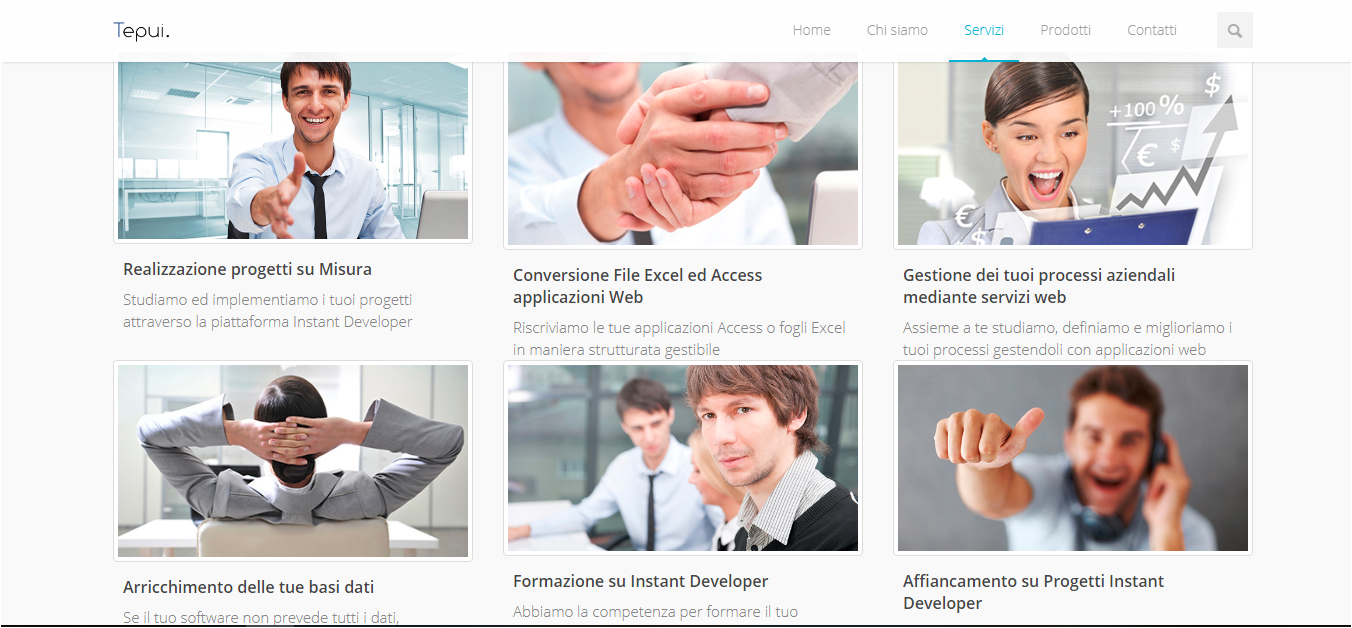
\includegraphics[width=0.8\columnwidth]{immagineServizi} 
	\caption{Prodotti e servizi forniti nella loro pagina web}
\end{figure}

\azienda\ persegue due diverse soluzioni per la creazione dei prodotti software: a pacchetto e su misura. Le soluzioni a pacchetto consistono in software completi già disponibili all'interno dell'azienda destinati alla vendita. Tuttavia, la loro vendita non è immediata ma segue comunque un controllo e modifica per adattare il prodotto venduto alla realtà del cliente. L'altro tipo di soluzione consiste, invece, nella realizzazione da zero di un prodotto. Questo tipo di servizio prevede tutti i passaggi dallo studio del problema alla realizzazione del prodotto completo.

Infine, per quanto riguarda i servizi, l'azienda fornisce la manutenzione di un qualsiasi prodotto InDe, sia esso creato da \azienda\ o da una qualsiasi altra ditta che faccia affidamento a tale piattaforma, purché si disponga del codice sorgente. Inoltre, tra i servizi offerti troviamo anche: formazione su InDe, affiancamento ai progetti con InDe, conversione dei file Excel ed Access in applicazioni web e la possibilità di sfruttare prodotti web per i processi aziendali \hyperref[bib1]{\cite{[1]}}.


\subsection{Tecnologie di riferimento}
\label{cap1:Tecnologie di riferimento}
\subsubsection*{Linguaggi di programmazione}

L'azienda opera nell'ambito web. I prodotti realizzati si basano sui seguenti linguaggi di programmazione lato server: 
\begin{itemize}
	\item \textbf{C\#}: linguaggio di programmazione orientato agli oggetti che consente di creare una vasta gamma di applicazioni protette e affidabili per .NET Framework. Esso può essere adottato per creare applicazioni client Windows, servizi Web XML, componenti distribuiti, applicazioni client\-server, applicazioni di database e molto altro \hyperref[bib3]{\cite{[3]}}.
	
	\item \textbf{Java}: ``linguaggio di programmazione ad alto livello, orientato agli oggetti e a tipizzazione statica, che si appoggia sull'omonima piattaforma software, specificamente progettato per essere il più possibile indipendente dalla piattaforma hardware di esecuzione'' \footnote[1]{\hyperref[bib4]{[4]}}.
\end{itemize}

Per quanto riguarda la componente grafica, le tecnologie adottate sono: HTML5, CSS3 e Javascript.

\begin{figure}[!h] 
	\centering 
	\includegraphics[width=0.7\columnwidth]{Tecnologie} 
	\caption{Linguaggi di programmazione}
	\label{tecnologie}
\end{figure}

\subsubsection*{Database}
Tutte le applicazioni dell'azienda mirano alla realizzazione di software gestionale, i quali necessitano di uno o più database, o per realtà più grandi dei Data Warehouse. I principali  database che hanno avuto modo di incontrare nello svolgimento delle loro attività sono stati: MySql, DB2, PostgreSQL, Oracle e SQL Server.\\

Tra i differenti database disponibili, quello adottato \azienda\ è principalmente SQL Server. La scelta ricade su questo dispositivo perché rappresenta un punto di incontro tra prestazioni, flessibilità e costi \hyperref[bib5]{\cite{[5]}}.\\
Altri fattori degni di nota riguardano il suo elevato utilizzo da parte delle aziende del territorio e per la sua popolarità visto che ancora oggi risulta essere il terzo database più usato al mondo dopo Oracle e MySQL \hyperref[bib6]{\cite{[6]}}. 

\begin{figure}[!h] 
	\centering 
	
\includegraphics[width=0.8\columnwidth]{database} 
	\caption{Database}
\end{figure}


\section{Processi aziendali}
\label{cap1:Processi aziendali}

Questa sezione presenta l'organizzazione dell'azienda e come quest'ultima cerchi di migliorarsi nel corso del tempo. 

\subsection{Miglioramento della qualità dei processi}
\label{cap1:Miglioramento della qualità dei processi}

\azienda\ nello svolgimento delle proprie attività opta per perseguire il costante miglioramento dei processi. Per fare questo fa affidamento al ciclo PDCA che si compone di quattro attività:
\begin{itemize}
	\item \textbf{P}lan: individuazione degli obiettivi di miglioramento e creazione di un piano d'azione nello svolgimento dei lavori;
	\item \textbf{D}o: esecuzione di quanto pianificato;
	\item \textbf{C}heck: analisi dei risultati ottenuti nella fase precedente e confronto con quanto pianificato; 
	\item \textbf{A}ct: standardizzazione delle attività andate a buon fine e rielaborazione di quelle da migliorare ricominciando con la pianificazione.
\end{itemize}

\begin{figure}[!h] 
	\centering 
	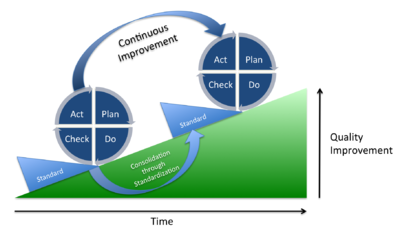
\includegraphics[width=0.8\columnwidth]{PDCA} 
	\caption{Ciclo PDCA (\url{https://bit.ly/2y3khfp})}
\end{figure}

Durante lo stage, ho notato che l'azienda adotta questa strategia principalmente nel processo di sviluppo mirando ad ottenere un prodotto efficiente ed efficacie. Negli altri processi aziendali invece, quali ad esempio la documentazione, spesso viene volontariamente scelto di dargli un importanza marginale. Questa decisione è legato al software che in alcuni casi si presta alla prototipizzazione rapida (\hyperref[cap1:Metodologia agile]{Sezione \ref{cap1:Metodologia agile}}), discussione con il cliente e successiva revisione. 
 
% La documentazione realizzata non è sempre completa. Viene preferito affidarsi ai mock\-up ed ai documenti che descrivono le caratteristiche tecniche e grafiche del prodotto in maniera poco completa, quando l'ideale sarebbe indagare su questi punti, ma in maniera più dettagliata fin dall'inizio. Infatti, nel corso del progetto mi sono trovato diverse volte a chiedere informazioni al tutor aziendale (responsabile di progetto), in merito a delle funzionalità non espresse nei documenti redatti e a me consegnati.  

\subsection{Metodologia agile}
\label{cap1:Metodologia agile}

L'azienda nello sviluppo delle applicazioni adotta la metodologia agile. \\
Questo metodo operativo permette una maggiore libertà rispetto ad altri tipi quali sequenziale, incrementale o a spirale. I punti fondamentali sono:
\begin{itemize}
	\item privilegiare la realizzazione del software alla creazione di documentazione;
	\item collaborare con il cliente invece di dedicarsi a contrattazioni;
	\item essere pronti a reagire ad ogni situazione invece di avere un piano di gestione dei rischi.
\end{itemize}
\azienda\ ha deciso di adottare questo metodo lavorativo per i suoi prodotti perché hanno osservato come nella realtà lavorativa le aziende vorrebbero avere a disposizione prodotti efficienti ed efficaci in tempi molto brevi. 
Inoltre, la scelta è ricaduta su questa tipologia per un motivo molto importante: conoscere i clienti, il mercato e creare un rapporto duraturo di fiducia. 

Questo metodo si concretizza con degli incontri la cui scadenza può essere, settimanale, bisettimanale o mensili, con i clienti.\\
Durante gli incontri si raccolgono task, migliorie da apportare ai progetti o addirittura ci si ferma dal cliente per realizzare nuove funzionalità e chiedere informazioni in maniera immediata. Così facendo la comunicazione è rapida, le mail sono ridotte ed è molto più facile comprendere le necessità delle aziende clienti osservandole dall'intero.


\section{Strumenti a supporto dei processi}
\label{cap1:Strumenti a supporto dei processi}
Questa sezione illustra gli strumenti adoperati a supporto dei processi e per lo sviluppo mirati a garantire qualità dei prodotti e servizi.

\subsection{Gestione di progetto}
\label{cap1:Gestione di progetto}

La gestione di progetto consiste nel definire ed organizzare il lavoro da svolgere in tempi e modi ben definiti. Per il seguente processo vengono utilizzati tre strumenti: Microsoft Teams, iDo e le mail.

\paragraph{Micorsoft Teams} è un'applicazione di comunicazione unificata multi-piattaforma . Essa permette di creare diversi gruppi con all'interno molti canali di comunicazione ai quali possono accedere solo le persone invitate. L'azienda crea un gruppo per ogni cliente e all'interno prevede un canale generale dove inserire documentazione o fare domande di natura generica. Mentre gli altri riguardano un progetto specifico o le singole funzionalità da implementare, se vi è un unico progetto. 

\begin{figure}[!h] 
	\centering 
	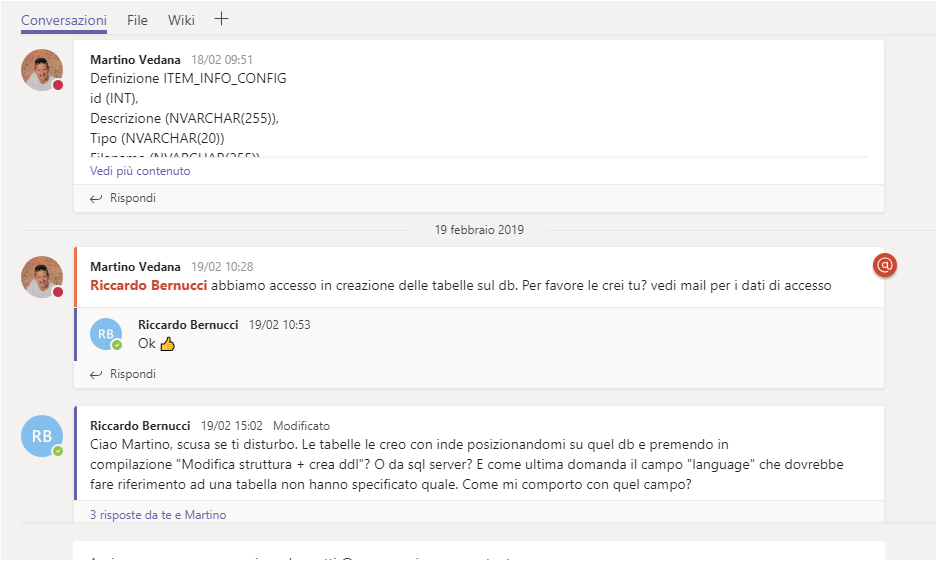
\includegraphics[height=0.4\columnwidth]{Teams} 
	\caption{Conversazione su Teams}
\end{figure}


\paragraph{Mail} ovvero la posta elettronica. Per iniziare il progetto mi è stata fornita una mail aziendale. Le mail servono per comunicare in maniera tempestiva la creazione ed assegnazione di una commessa nell'applicazione iDo. Queste ultime sono il principale mezzo di comunicazione con le aziende clienti. Una prassi interna all'azienda prevede che per informazioni da chiedere al cliente, bisogna prima discuterne internamente tra i membri del gruppo assegnato a quel progetto e poi quella di mettere in copia carbone il responsabile di progetto alla eventuale mail da inviare ai clienti.



\paragraph{iDo} è un'applicazione web realizzata con InDe dove vengono assegnate le commesse, indicando tempi di inizio e fine previsti. In questo applicativo, si devono indicare le ore svolte dai lavoratori specificando le ore di inizio, fine e informazioni di quanto si è svolto in quel periodo. Inoltre, si possono inserire commenti utili all'azienda cliente e a \azienda. 
Grazie a questa applicazione viene calcolato il compenso e il consuntivo del progetto. Essa si compone di diverse sezioni la Kanban (\hyperref[ido]{figura \ref{ido}}), dove vengono presentate tutte le commesse con in testa il nome del cliente e del progetto; una sezione Commessa, nella quale vengono inseriti i progetti assegnati e navigando al suo interno si accede alle commesse; una sezione tempi, dedicata a sistemare eventuali errori di inserimento a fine mese o per controllare le attività svolte dai dipendenti e prendere le opportune decisioni.

\begin{figure}[!h] 
	\centering 
	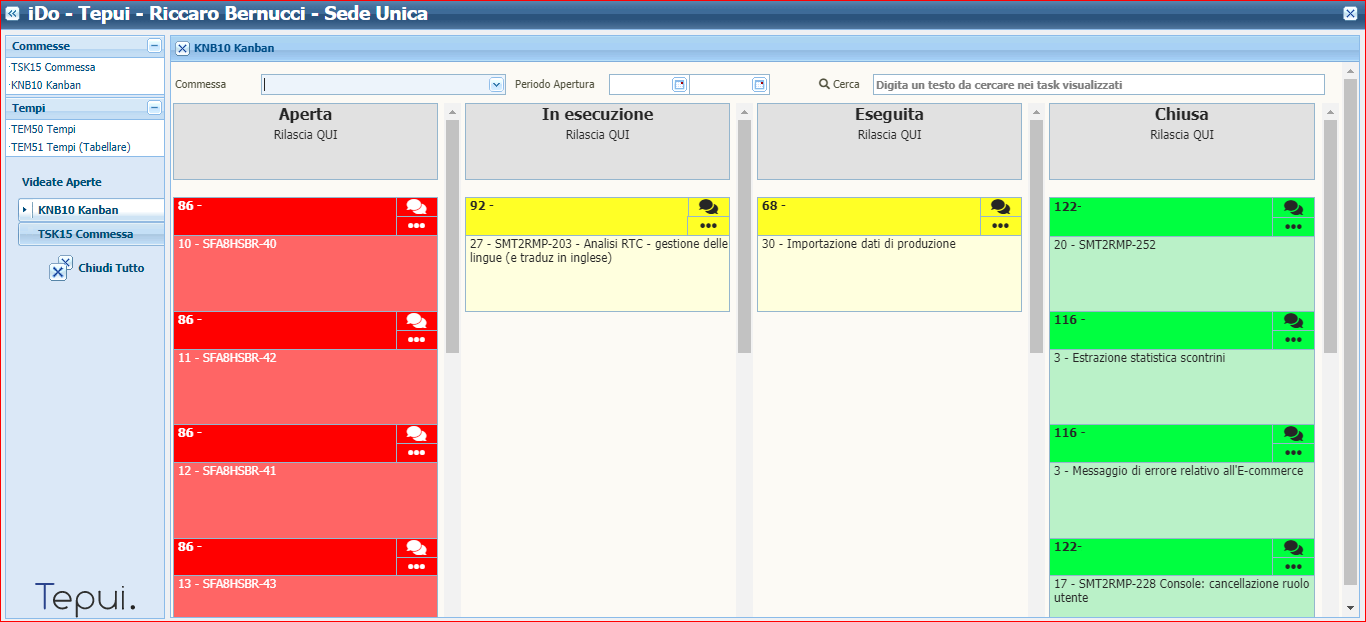
\includegraphics[width=0.8\columnwidth]{iDo} 
	\caption{Kanban dell'applicazione iDo (con nome cliente censurato)}
	\label{ido}
\end{figure}



\subsection{Documentazione}
\label{cap1:Documentazione}

L'azienda, sebbene abbia deciso di adottare un modello agile, non è priva di documenti. Quando deve realizzare un progetto il primo passo è quello di redigere un Piano di progetto e un POC documentale con le principali caratteristiche del prodotto finale. 
Il motivo per cui la società dà molta importanza al POC è che, con un documento nel quale è riportato la struttura del database e la grafica pressapochista del progetto, è possibile realizzare un prodotto completo in 3/4 settimane. 
La documentazione è salvata interamente su OneDrive For Business. Ogni documento ha una sua collocazione da rispettare. 

\subsection{Sistema di versionamento}
\label{cap1:Sistema di versionamento}

Per il versionamento e il salvataggio dei file prodotti durante la realizzazione dei progetti è previsto l'utilizzo di una repository creata dal Project Manager su un'applicazione web ideato sempre su InDe, TeamWorks. Successivamente, vengono forniti ai dipendenti scelti nella realizzazione di uno specifico progetto i permessi di: scrittura, lettura ed eliminazione.
Questa applicazione web risulta essere molto simile a GitHub, tuttavia è molto più intuitivo e semplice perché le funzionalità permesse sono visualizzare le informazioni relative ai commit, tornare indietro di versione (rollback), scaricare progetti (Download) e creare dei derivati (Fork) premendo unicamente dei pulsanti.

Ciascun progetto deve essere soggetto a versionamento perciò chiunque lo utilizza ha una visione chiara e dettagliata della sua storia e delle sue modifiche. Ad ogni task deve corrispondere una versione. Nelle versioni viene applicato il seguente formalismo:
\begin{center}
	X.Y.Z
\end{center}
Dove X,Y,Z sono numeri incrementali da 0 a infinito. 
Z indica i singoli task e bug da risolvere implementati, Y rappresenta il corretto funzionamento delle nuove funzionalità rilasciate per la fase di verifica e collaudo e X quando il progetto ha superato tutti i controlli e diventa operativo.  

\subsubsection{Sistema di pubblicazione}
La pubblicazione presso \azienda\ corrisponde al rilascio dell'applicazione al cliente per effettuare dei test. Il collaudo viene effettuato anche internamente all'azienda, ma questa doppio controllo permette di realizzare applicazioni corrette che non necessitino di eccessive manutenzioni di tipo correttivo. 
Il sistema adottato per pubblicare il software è IDManager, anche essa una applicazione web di InDe, la quale permette di modificare i riferimenti del database cambiando la stringa di connessione del progetto e permette di caricare unicamente le differenze tra la versione precedente e quella attuale.


\subsection{Ambiente di sviluppo}
\label{cap1:Ambiente di sviluppo}

\paragraph{\inde} consiste in una piattaforma ad alta produttività, per lo sviluppo di applicazioni cross-platform (Web-based) creata da Pro Gamma S.p.A.. La scelta dell'azienda ricade su questo tipo di strumento per i seguenti motivi \hyperref[bib1]{\cite{[1]}}:
\begin{itemize}
	\item Scrivere l'applicazione e poterla distribuire in ambiente Java o Microsoft C\#;
	\item Collegare ed utilizzare più database contemporaneamente anche di tipo differente;
	\item Implementare applicazioni Desktop e Mobile;
	\item Gestire i rilasci successivi in maniera sicura e strutturata;
	\item Potersi focalizzare sui processi da gestire, sui i dati da memorizzare o modificare, evitando di dover programmare a basso livello, avendo però la possibilità, quando necessario, di poterlo fare.
\end{itemize}
Le applicazioni prodotte sono multi-piattaforma, cross-browser, multi-database già nel momento in cui vengono create \hyperref[bib1]{\cite{[1]}}.

\paragraph{Microsoft SQL Server} Un DBMS relazionale, prodotto da Microsoft, che usa T-SQL, una variante del linguaggio SQL Standard \hyperref[bib7]{\cite{[7]}}. 

\paragraph{Microsoft SQL Server Management Studio} \'E un'applicazione software che viene utilizzata per la configurazione, la gestione e l'amministrazione di tutti i componenti all'interno di Microsoft SQL Server. Lo strumento include sia editor di script che strumenti grafici che funzionano con oggetti e funzionalità del server \hyperref[bib8]{\cite{[8]}}.

\paragraph{Qlik}\'E un pacchetto che include QlikView, Qlik Sense ed NPrinting. Questi software sono di visualizzazione e business intelligence che permettono il rapido sviluppo di dashboard completamente personalizzabili in grado di fornire rapidamente informazioni utili sui dati a disposizione \hyperref[bib9]{\cite{[9]}}.

\paragraph{Microsoft Power BI}
\'E un servizio di analisi aziendale di Microsoft fortemente integrato con Microsoft Office e con gli altri strumenti dell'ecosistema Microsoft. Mira a fornire visualizzazioni interattive e funzionalità di business intelligence con un'interfaccia abbastanza semplice in modo da consentire agli utenti finali di creare i propri report e dashboard \hyperref[bib10]{\cite{[10]}}.

\subsubsection*{Altri strumenti}
Oltre agli strumenti appena descritti, eventuali \hyperref[IDE]{IDE} per scrivere in C\#, Java e gli altri linguaggi riportati in Sezione \ref{cap1:Tecnologie di riferimento}, sono lasciati al programmatore. Può capitare che nel corso di un progetto siano richieste  modifiche specifiche che l'applicazione InDe non permette, in quei casi vi è una modalità di inserimento personalizzato che consente di scrivere codice.



\subsection{Sistemi operativi}
\label{cap1:Sistemi operativi}

L'azienda usa  solo i sistemi operativi di Windows. Questo perché risultano essere gli unici compatibili con InDe. Per chi non dovesse avere a disposizione tale sistema operativo viene fornita una macchina virtuale alla quale collegarsi. 

\subsubsection*{VPN e desktop remoto}
In base al progetto, spesso può capitare che ci si debba affidare alla macchina virtuale del cliente. In queste occasioni l'azienda consiglia l'utilizzo di una delle seguenti applicazioni per connettersi alla VPN: openVPN, FortiClient o lo strumento di Windows. 
Mentre per entrare in desktop remoto: Connessione Desktop Remoto di windows oppure nRemoteNG, il quale offre anche la possibilità di creare una o più connessione VPN ed aprire diversi schermi remoti contemporaneamente. 
Quando invece si effettuano delle assistenze, AnyDesk o TeamViewer sono dei software efficienti per collegarsi al desktop del cliente e risolvere problemi.


\section{Clientela}
\label{cap1:Clientela}
I clienti di \azienda\ risiedono nei territori del nord Italia. La sede legale dell'azienda si trova a Milano. A Castelfranco veneto è collocata una delle due sedi operative, presso la quale ho svolto la mia esperienza di stage.\\
I clienti sono imprese di medio-grandi dimensioni. Altre imprese degne di nota sono Aton s.p.a, Sistemi s.p.a, WiseEnergy Italia s.r.l, Geox s.p.a. ed altre aziende che operano a livello internazionale.

\paragraph*{}In seguito alla compilazione dell'\hyperref[NDA]{Accordo di non divulgazione} per l'intera durata del progetto non verrà nominato il nome dell'azienda cliente.

\newpage             % Introduzione
%% !TEX encoding = UTF-8
% !TEX TS-program = pdflatex
% !TEX root = ../tesi.tex

%**************************************************************
\chapter{Processi e metodologie}
\label{cap:processi-metodologie}
%**************************************************************

\intro{Brevissima introduzione al capitolo}\\

%**************************************************************
\section{Processo sviluppo prodotto}             % Processi
%% !TEX encoding = UTF-8
% !TEX TS-program = pdflatex
% !TEX root = ../tesi.tex

%**************************************************************
\chapter{Descrizione dello stage}
\label{cap:descrizione-stage}
%**************************************************************

\intro{Breve introduzione al capitolo}\\

%**************************************************************
\section{Introduzione al progetto}

%**************************************************************
\section{Analisi preventiva dei rischi}

Durante la fase di analisi iniziale sono stati individuati alcuni possibili rischi a cui si potrà andare incontro.
Si è quindi proceduto a elaborare delle possibili soluzioni per far fronte a tali rischi.\\

\begin{risk}{Performance del simulatore hardware}
    \riskdescription{le performance del simulatore hardware e la comunicazione con questo potrebbero risultare lenti o non abbastanza buoni da causare il fallimento dei test}
    \risksolution{coinvolgimento del responsabile a capo del progetto relativo il simulatore hardware}
    \label{risk:hardware-simulator} 
\end{risk}

%**************************************************************
\section{Requisiti e obiettivi}


%**************************************************************
\section{Pianificazione}             % Piano di progetto (preventivi effettuati) - Kick-Off
%% !TEX encoding = UTF-8
% !TEX TS-program = pdflatex
% !TEX root = ../tesi.tex

%**************************************************************
\chapter{Analisi dei requisiti}
\label{cap:analisi-requisiti}
%**************************************************************

\intro{Breve introduzione al capitolo}\\

\section{Casi d'uso}

Per lo studio dei casi di utilizzo del prodotto sono stati creati dei diagrammi.
I diagrammi dei casi d'uso (in inglese \emph{Use Case Diagram}) sono diagrammi di tipo \gls{uml} dedicati alla descrizione delle funzioni o servizi offerti da un sistema, così come sono percepiti e utilizzati dagli attori che interagiscono col sistema stesso.
Essendo il progetto finalizzato alla creazione di un tool per l'automazione di un processo, le interazioni da parte dell'utilizzatore devono essere ovviamente ridotte allo stretto necessario. Per questo motivo i diagrammi d'uso risultano semplici e in numero ridotto.

\begin{figure}[!h] 
    \centering 
    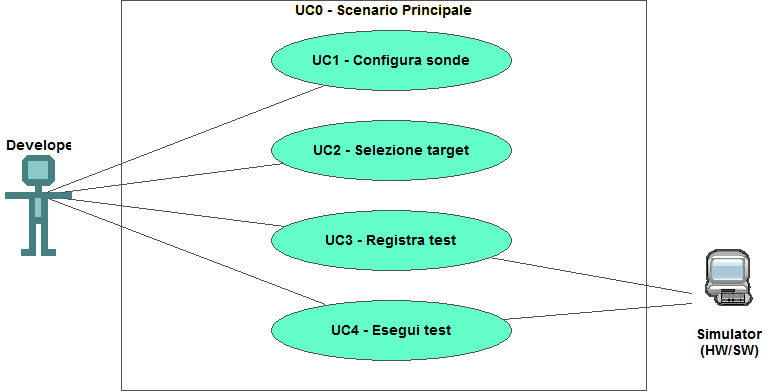
\includegraphics[width=0.9\columnwidth]{usecase/scenario-principale} 
    \caption{Use Case - UC0: Scenario principale}
\end{figure}

\begin{usecase}{0}{Scenario principale}
\usecaseactors{Sviluppatore applicativi}
\usecasepre{Lo sviluppatore è entrato nel plug-in di simulazione all'interno dell'IDE}
\usecasedesc{La finestra di simulazione mette a disposizione i comandi per configurare, registrare o eseguire un test}
\usecasepost{Il sistema è pronto per permettere una nuova interazione}
\label{uc:scenario-principale}
\end{usecase}

\section{Tracciamento dei requisiti}

Da un'attenta analisi dei requisiti e degli use case effettuata sul progetto è stata stilata la tabella che traccia i requisiti in rapporto agli use case.\\
Sono stati individuati diversi tipi di requisiti e si è quindi fatto utilizzo di un codice identificativo per distinguerli.\\
Il codice dei requisiti è così strutturato R(F/Q/V)(N/D/O) dove:
\begin{enumerate}
	\item[R =] requisito
    \item[F =] funzionale
    \item[Q =] qualitativo
    \item[V =] di vincolo
    \item[N =] obbligatorio (necessario)
    \item[D =] desiderabile
    \item[Z =] opzionale
\end{enumerate}
Nelle tabelle \ref{tab:requisiti-funzionali}, \ref{tab:requisiti-qualitativi} e \ref{tab:requisiti-vincolo} sono riassunti i requisiti e il loro tracciamento con gli use case delineati in fase di analisi.

\newpage

\begin{table}%
\caption{Tabella del tracciamento dei requisti funzionali}
\label{tab:requisiti-funzionali}
\begin{tabularx}{\textwidth}{lXl}
\hline\hline
\textbf{Requisito} & \textbf{Descrizione} & \textbf{Use Case}\\
\hline
RFN-1     & L'interfaccia permette di configurare il tipo di sonde del test & UC1 \\
\hline
\end{tabularx}
\end{table}%

\begin{table}%
\caption{Tabella del tracciamento dei requisiti qualitativi}
\label{tab:requisiti-qualitativi}
\begin{tabularx}{\textwidth}{lXl}
\hline\hline
\textbf{Requisito} & \textbf{Descrizione} & \textbf{Use Case}\\
\hline
RQD-1    & Le prestazioni del simulatore hardware deve garantire la giusta esecuzione dei test e non la generazione di falsi negativi & - \\
\hline
\end{tabularx}
\end{table}%

\begin{table}%
\caption{Tabella del tracciamento dei requisiti di vincolo}
\label{tab:requisiti-vincolo}
\begin{tabularx}{\textwidth}{lXl}
\hline\hline
\textbf{Requisito} & \textbf{Descrizione} & \textbf{Use Case}\\
\hline
RVO-1    & La libreria per l'esecuzione dei test automatici deve essere riutilizzabile & - \\
\hline
\end{tabularx}
\end{table}%             % Analisi dei requisiti - Concept Preview
%% !TEX encoding = UTF-8
% !TEX TS-program = pdflatex
% !TEX root = ../tesi.tex

%**************************************************************
\chapter{Progettazione e codifica}
\label{cap:progettazione-codifica}
%**************************************************************

\intro{Breve introduzione al capitolo}\\

%**************************************************************
\section{Tecnologie e strumenti}
\label{sec:tecnologie-strumenti}

Di seguito viene data una panoramica delle tecnologie e strumenti utilizzati.

\subsection*{Tecnologia 1}
Descrizione Tecnologia 1.

\subsection*{Tecnologia 2}
Descrizione Tecnologia 2

%**************************************************************
\section{Ciclo di vita del software}
\label{sec:ciclo-vita-software}

%**************************************************************
\section{Progettazione}
\label{sec:progettazione}

\subsubsection{Namespace 1} %**************************
Descrizione namespace 1.

\begin{namespacedesc}
    \classdesc{Classe 1}{Descrizione classe 1}
    \classdesc{Classe 2}{Descrizione classe 2}
\end{namespacedesc}


%**************************************************************
\section{Design Pattern utilizzati}

%**************************************************************
\section{Codifica}
             % Progettazione e codifica - Product Prototype
%% !TEX encoding = UTF-8
% !TEX TS-program = pdflatex
% !TEX root = ../tesi.tex

%**************************************************************
\chapter{Verifica e validazione}
\label{cap:verifica-validazione}
%**************************************************************             % Verifica e Validazione - Product Design Freeze e SOP
%% !TEX encoding = UTF-8
% !TEX TS-program = pdflatex
% !TEX root = ../tesi.tex

%**************************************************************
\chapter{Conclusioni}
\label{cap:conclusioni}
%**************************************************************

%**************************************************************
\section{Consuntivo finale}

%**************************************************************
\section{Raggiungimento degli obiettivi}

%**************************************************************
\section{Conoscenze acquisite}

%**************************************************************
\section{Valutazione personale}
             % Conclusioni
%\appendix                               
%% !TEX encoding = UTF-8
% !TEX TS-program = pdflatex
% !TEX root = ../tesi.tex

%**************************************************************
\chapter{Appendice A}
%**************************************************************

\epigraph{Citazione}{Autore della citazione}



             % Appendice A

%**************************************************************
% Materiale finale
%**************************************************************
\backmatter
\chapter{Glossario}
\paragraph{API} 
\label{API} 
In informatica con il termine \emph{Application Programming Interface API} (ing. interfaccia di programmazione di un'applicazione) si indica ogni insieme di procedure disponibili al programmatore, di solito raggruppate a formare un set di strumenti specifici per l'espletamento di un determinato compito all'interno di un certo programma. La finalità è ottenere un'astrazione, di solito tra l'hardware e il programmatore o tra software a basso e quello ad alto livello semplificando così il lavoro di programmazione

\paragraph{UML} 
\label{UML} 
In ingegneria del software \emph{UML, Unified Modeling Language} (ing. linguaggio di modellazione unificato) è un linguaggio di modellazione e specifica basato sul paradigma object-oriented. L'\emph{UML} svolge un'importantissima funzione di ``lingua franca'' nella comunità della progettazione e programmazione a oggetti. Gran parte della letteratura di settore usa tale linguaggio per descrivere soluzioni analitiche e progettuali in modo sintetico e comprensibile a un vasto pubblico

\paragraph{C\#}
Linguaggio di programmazione orientato agli oggetti che consente di creare una vasta gamma di applicazioni protette e affidabili per .NET Framework. Esso può essere adottato per creare applicazioni client Windows, servizi Web XML, componenti distribuiti, applicazioni client\-server, applicazioni di database e molto altro.

\paragraph{Java}
Linguaggio di programmazione ad alto livello, orientato agli oggetti e a tipizzazione statica, che si appoggia sull'omonima piattaforma software, specificamente progettato per essere il più possibile indipendente dalla piattaforma hardware di esecuzione.

\paragraph{IDE}
\label{IDE}
Un ambiente di sviluppo integrato (in lingua inglese Integrated Development Environment), è un software che, in fase di programmazione, aiuta i programmatori nello sviluppo del codice sorgente di un programma. 
Spesso l'IDE aiuta lo sviluppatore segnalando errori di sintassi del codice direttamente in fase di scrittura, oltre a tutta una serie di strumenti e funzionalità di supporto alla fase di sviluppo e debugging.

\paragraph{Accordo di non divulgazione}
\label{NDA}
Un accordo di non divulgazione (in lingua inglese Non-Disclosure Agreement, NDA) è un negozio giuridico di natura sinallagmatica che designa informazioni confidenziali e con il quale le parti si impegnano a mantenerle segrete, pena la violazione dell'accordo stesso e il decorso di specifiche clausole penali in esso contenute.

\paragraph{Instant Developer}
\label{InDe}
Instant Developer, in particolare la versione per desktop, Foundation è la piattaforma di sviluppo adottata per creare il progetto oggetto della tesi. Si tratta di un RAD che permette di realizzare applicazioni in tempi molto brevi senza la necessità di conoscere il codice alla base del progetto. 

\chapter{Acronimi e abbreviazioni}

\noindent \hyperref[UMLl]{UML - Unified Modeling Language}
\\
\\
\noindent \hyperref[IDE]{IDE - Integrated Development Environment}
\\
\\
\noindent \hyperref[NDA]{NDA - Non-Disclosure Agreement}
\\
\\
\noindent \hyperref[InDe]{InDe - Instant Developer}
\\
\\
\noindent \hyperref[OOP]{OOP - Object Oriented Programming}
\\
\\
\noindent \hyperref[DO]{DO - Document Oriented}
\\
\\
\noindent \hyperref[TO]{TO - Table Oriented}
\\
\\
\noindent \hyperref[RAD]{RAD - Rapid Application Development}
\\
\\
\noindent \hyperref[CASE]{CASE - Computer Aided Software Engineering}
\\
\\
\noindent \hyperref[ORM]{ORM - Object Relational Mapping}
\\
\\

% !TEX encoding = UTF-8
% !TEX TS-program = pdflatex
% !TEX root = ../tesi.tex

%**************************************************************
% Bibliografia
%**************************************************************

\cleardoublepage
\chapter{Fonti}

%Inserire bibliografie
\section*{Bibliografia}

%inserire sitografia
\section*{Sitografia}
\begin{itemize}
	\item \textit{Informazioni sull'azienda - consultato 23/05/2019}\\
	\url{https://www.tepui.it/servizi/}
	
	\item \textit{Definizione di Software gestionale - consultato 23/05/2019}\\
	\url{https://bit.ly/2H8Cr4P}
	
	\item \textit{Definizione di C\# - Consultato 23/05/2019}\\
	\url{https://bit.ly/308zwjY}
	
	\item \textit{Definizione di Java - Consultato 23/05/2019}\\
	\url{https://bit.ly/1dHppDG} 
	
	\item \textit{Definizione di Qlik - Consultato 23/05/2019}\\
	\url{https://bit.ly/2J76agL} 
	
	\item \textit{Definizione di SSMS - Consultato 23/05/2019}\\
	\url{https://bit.ly/2VPWZHn} 
	
	\item \textit{Definizione di Microsoft Power BI - Consultato 23/05/2019}\\
	\url{https://bit.ly/2FkLBeX}
	
	\item \textit{Definizione di IDE - Consultato 23/05/2019}\\
	\url{https://bit.ly/2Ozruuv}
	
	\item \textit{Definizione di NDA - Consultato 23/05/2019}\\
	\url{https://bit.ly/2Lw4sYu}
	
	\item \textit{Scegliere SQL Server - Consultato 09/07/2019}\\
	\url{https://bit.ly/2YJ3RVt}
	
	\item \textit{Statistiche SQL Server - Consultato 09/07/2019}\\
	\url{https://bit.ly/2XxEjhv}
	
	
\end{itemize}






\end{document}
